
\documentclass[crop]{standalone}% 'crop' is the default for v1.0, before it was 'preview'
%\usetikzlibrary{...}% tikz package already loaded by 'tikz' option
\usepackage[usenames,dvipsnames]{xcolor}
\usepackage{tikz,pgfplots}
\usetikzlibrary{backgrounds}
\usetikzlibrary{external,calc,patterns,decorations.pathmorphing}
\usetikzlibrary{positioning,pgfplots.fillbetween}
\usetikzlibrary {patterns.meta}
\pgfplotsset{compat=1.17}
\usepackage{accents}
\begin{document}
	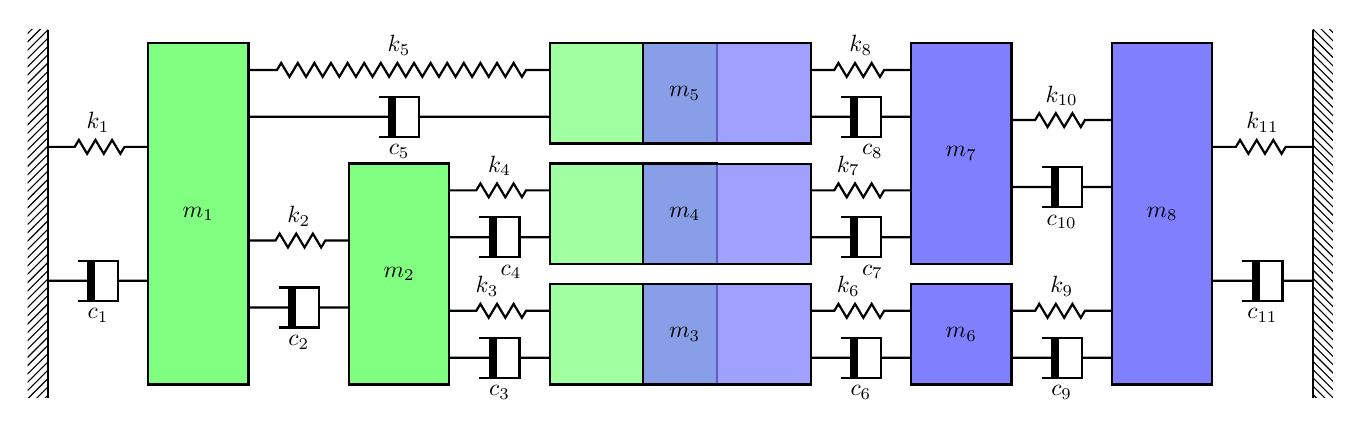
\begin{tikzpicture}[scale=0.85,every node/.style={outer sep=0pt,transform shape},thick,
		mass/.style={draw,thick},
		spring/.style={thick,decorate,decoration={zigzag,pre length=0.3cm,post
				length=0.3cm,segment length=6}},
		groundL/.style={fill,pattern=north east lines,draw=none,minimum
			width=0.75cm,minimum height=0.3cm},
		groundR/.style={fill,pattern=north west lines,draw=none,minimum
			width=0.75cm,minimum height=0.3cm},
		dampic/.pic={\fill[white] (-0.1,-0.3) rectangle (0.3,0.3);
			\draw (-0.3,0.3) -| (0.3,-0.3) -- (-0.3,-0.3);
			\draw[line width=1mm] (-0.1,-0.3) -- (-0.1,0.3);}]
		
		
		%%%%%%%%%%%%%% SUB SYSTEM A %%%%%%%%%%%%%%%%%%
		%% GROUND L
		\node[groundL,minimum width=3mm,minimum height=5.5cm] (g1){};
		\draw (g1.north east) -- (g1.south east);
		
		%% MASS 1
		\node[mass,minimum width=1.5cm,minimum height=5.1cm,fill=green!50!white,right=1.5cm of g1] (m1) {$m_1$};  
		%% MASS 2  
		\node[mass,minimum width=1.5cm,minimum height=3.3cm,fill=green!50!white,below right=-3.3cm and 1.5cm of m1] (m2) {$m_2$}; 
		%% MASS 3 
		\node[mass,minimum width=2.5cm,fill opacity = 0.75,minimum height=1.5cm,fill=green!50!white,below right=-1.5cm and 1.5cm of m2] (m3) {};  
		%% MASS 4 
		\node[mass,minimum width=2.5cm,fill opacity = 0.75,minimum height=1.5cm,fill=green!50!white,above right=-1.5cm and 1.5cm of m2] (m4) {};
		%% MASS 5
		\node[mass,minimum width=2.5cm,fill opacity = 0.75,minimum height=1.5cm,fill=green!50!white,above right=-1.5cm and 4.5cm of m1] (m5) {};
		
		%% SPRINGS
		\draw[spring] ([yshift=1cm]m1.west) coordinate(aux)-- (g1.east|-aux)  node[midway,above=1mm]{$k_1$};  
		\draw[spring]  ([yshift=0.5cm]m2.west) coordinate(aux) -- (m1.east|-aux) node[midway,above=1mm]{$k_2$};  
		\draw[spring]  ([yshift=0.35cm]m3.west) coordinate(aux) -- (m2.east|-aux) node[midway,above left=1mm and -1mm]{$k_3$};
		\draw[spring]  ([yshift=0.35cm]m4.west) coordinate(aux) -- (m2.east|-aux) node[midway,above=1mm]{$k_4$};       
		\draw[spring]  ([yshift=0.35cm]m5.west) coordinate(aux) -- (m1.east|-aux) node[midway,above=1mm]{$k_5$};
		
		%% DAMPERS
		\draw ([yshift=-1cm]m1.west) coordinate(aux)-- (g1.east|-aux)   pic[midway]{dampic} node[midway,below=3mm]{$c_1$};     
		\draw ([yshift=-0.5cm]m2.west) coordinate(aux)-- (m1.east|-aux)   pic[midway]{dampic} node[midway,below=3mm]{$c_2$};   
		\draw ([yshift=-0.35cm]m3.west) coordinate(aux)-- (m2.east|-aux)   pic[midway]{dampic} node[midway,below=3mm]{$c_3$}; 
		\draw ([yshift=-0.35cm]m4.west) coordinate(aux)-- (m2.east|-aux)   pic[midway]{dampic} node[midway,below right=3mm and -1mm]{$c_4$}; 
		\draw ([yshift=-0.35cm]m5.west) coordinate(aux)-- (m1.east|-aux)   pic[midway]{dampic} node[midway,below=3mm]{$c_5$}; 
		
		
		%%%%%%%%%%%%%% SUB SYSTEM B %%%%%%%%%%%%%%%%%%
		%% GROUND R
		\node[right=18.9cm of g1,groundR,minimum width=3mm,minimum height=5.5cm] (g2){};
		\draw (g2.north west) -- (g2.south west)  ;
		
		%% MASS 1
		\node[mass,minimum width=1.5cm,minimum height=5.1cm,fill=blue!50!white,left=1.5cm of g2] (m11) {$m_{8}$};  
		%% MASS 2  
		\node[mass,minimum width=1.5cm,minimum height=1.5cm,fill=blue!50!white,below left=-1.5cm and 1.5cm of m11] (m9) {$m_{6}$}; 
		%% MASS 2  
		\node[mass,minimum width=1.5cm,minimum height=3.3cm,fill=blue!50!white,above left=-3.3cm and 1.5cm of m11] (m10) {$m_{7}$}; 
		%% MASS 2  
		\node[mass,minimum width=2.5cm,minimum height=1.5cm,fill opacity=0.75,fill=blue!50!white,above left=-1.5cm and 1.5cm of m10] (m8) {}; 
		\node[mass,minimum width=2.5cm,fill opacity=0.75,minimum height=1.5cm,fill=blue!50!white,below left=-1.5cm and 1.5cm of m10] (m7) {}; 
		\node[mass,minimum width=2.5cm,fill opacity=0.75,minimum height=1.5cm,fill=blue!50!white,left=1.5cm of m9] (m6) {}; 
		\node [xshift=-18]at (m6) {$m_{3}$}; 
		\node [xshift=-18]at (m7) {$m_{4}$}; 		
		\node [xshift=-18]at (m8) {$m_{5}$}; 		
		%% SPRINGS
		\draw[spring] ([yshift=1cm]m11.east) coordinate(aux)-- (g2.west|-aux)  node[midway,above=1mm]{$k_{11}$};  
		\draw[spring] ([yshift=0.35cm]m9.east) coordinate(aux)-- (m11.west|-aux)  node[midway,above=1mm]{$k_{9}$};       
		\draw[spring] ([yshift=0.5cm]m10.east) coordinate(aux)-- (m11.west|-aux)  node[midway,above=1mm]{$k_{10}$};      
		\draw[spring] ([yshift=0.35cm]m7.east) coordinate(aux)-- (m10.west|-aux)  node[midway,above left=1mm and -1mm]{$k_{7}$};    \draw[spring] ([yshift=0.35cm]m8.east) coordinate(aux)-- (m10.west|-aux)  node[midway,above=1mm]{$k_{8}$};        
		\draw[spring] ([yshift=0.35cm]m6.east) coordinate(aux)-- (m9.west|-aux)  node[midway,above left=1mm and -1mm]{$k_{6}$};  
		
		%% DAMPERS
		\draw ([yshift=-1cm]m11.east) coordinate(aux)-- (g2.west|-aux)   pic[midway]{dampic} node[midway,below=3mm]{$c_{11}$};     
		\draw ([yshift=-0.5cm]m10.east) coordinate(aux)-- (m11.west|-aux)   pic[midway]{dampic} node[midway,below=3mm]{$c_{10}$}; 
		\draw ([yshift=-0.35cm]m9.east) coordinate(aux)-- (m11.west|-aux)   pic[midway]{dampic} node[midway,below=3mm]{$c_{9}$};  
		\draw ([yshift=-0.35cm]m6.east) coordinate(aux)-- (m9.west|-aux)   pic[midway]{dampic} node[midway,below=3mm]{$c_{6}$};  
		\draw ([yshift=-0.35cm]m7.east) coordinate(aux)-- (m10.west|-aux)   pic[midway]{dampic} node[midway,below right=3mm and -1mm]{$c_{7}$};  
		\draw ([yshift=-0.35cm]m8.east) coordinate(aux)-- (m10.west|-aux)   pic[midway]{dampic} node[midway,below right=3mm and -1mm]{$c_{8}$};  
		
		
		%%%%%%% CONNECTIONS %%%%%%%%%%%%%
%		\draw[ultra thick,dashed,red] (m5.east) coordinate(aux)-- (m8.west|-aux)  node[midway,above=1mm]{$\gamma_{3}$}; 
%		\node[mark size=2pt,color=red] at (m5.east) {\pgfuseplotmark{*}};
%		\node[mark size=2pt,color=red] at (m8.west|-aux) {\pgfuseplotmark{*}};
%		
%		\draw[ultra thick,dashed,red] (m4.east) coordinate(aux)-- (m7.west|-aux)  node[midway,above=1mm]{$\gamma_{2}$}; 
%		\node[mark size=2pt,color=red] at (m4.east) {\pgfuseplotmark{*}};
%		\node[mark size=2pt,color=red] at (m7.west|-aux) {\pgfuseplotmark{*}};
%		
%		\draw[ultra thick,dashed,red] (m3.east) coordinate(aux)-- (m6.west|-aux)  node[midway,above=1mm]{$\gamma_{1}$}; 
%		\node[mark size=2pt,color=red] at (m3.east) {\pgfuseplotmark{*}};
%		\node[mark size=2pt,color=red] at (m6.west|-aux) {\pgfuseplotmark{*}};
		
	\end{tikzpicture}
\end{document}